\documentclass[a4paper]{article}
\usepackage[T1]{fontenc}
\usepackage[utf8]{inputenc}
\usepackage{lmodern}
\usepackage{amsmath,amssymb}
\usepackage[top=3cm,bottom=2cm,left=2cm,right=2cm]{geometry}
\usepackage{fancyhdr}
\usepackage{esvect,esint}
\usepackage{xcolor}
\usepackage{tikz}\usetikzlibrary{calc}

\parskip1em\parindent0pt\let\ds\displaystyle

\begin{document}

\pagestyle{fancy}
\fancyhf{}
\setlength{\headheight}{15pt}
\fancyhead[L]{Thermodynamique}\fancyhead[R]{Question 17}

% Énoncé
\begin{center}
	\large{\boldmath{\textbf{Détente de Joule-Thompson}}}
\end{center}

% Correction

Soit un système ouvert $\Sigma$ en écoulement stationnaire dans un tuyau possédant un étranglement.

\begin{minipage}{0.5\linewidth}
  Aucun des paramètres ne dépend du temps.\\
  On considère le système fermé à l'instant $t$ entre $AB$ et $CD$ et à l'instant $t+\mathrm{d}t$ entre $A'B'$ et $C'D'$\\
  $m_{ABCD}=m_{A'B'C'D'}$ et $m_{A'B'CD}=m_{A'B'CD}$ donc $\\\mathrm{d}_{CC'DD'}=\mathrm{d}m_{ABA'B'}$\\
  Donc $\rho_1V_1\mathrm{d}t S_1=\rho_2V_2\mathrm{d}t S_2=\mathrm{d}m$
\end{minipage}\hfill
\begin{minipage}{0.3\linewidth}
  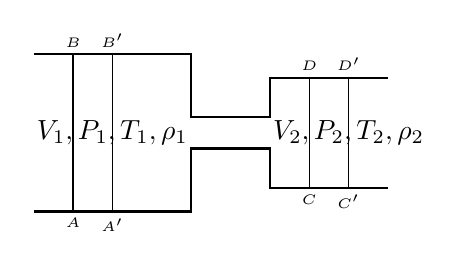
\begin{tikzpicture}
    \draw[thick] (0,0) -- (2,0) -- (2,0.8) -- ++(1,0) -- ++(0,-.5) -- ++(1.5,0) ++(0,1.4) -- ++(-1.5,0) -- ++(0,-.5) -- ++(-1,0) -- (2,1.2) -- (2,2) -- (0,2);
    \node at (1,1) {$V_1,P_1,T_1,\rho_1$};
    \node at (4,1) {$V_2,P_2,T_2,\rho_2$};
    {\tiny
    \draw (.5,0) node[below]{$A$} -- ++(0,2) node[above]{$B$};
    \draw (1,0) node[below]{$A'$} -- ++(0,2) node[above]{$B'$};
    \draw (3.5,.3
    ) node[below]{$C$} -- ++(0,1.4) node[above]{$D$};
    \draw (4,.3) node[below]{$C'$} -- ++(0,1.4) node[above]{$D'$};
    }
  \end{tikzpicture}
\end{minipage}\par

  Premier principe : $(U+E)_{A'B'C'D'}(t+\mathrm{d}t)-(U+E)_{ABCD}(t)=\delta W+\delta W_u+\delta Q$ où $\delta W$ est le travail des forces de pression et $\delta W_u$ est le travail du reste.\\
  $\delta W=\Delta(PSV\mathrm{d}t)=\mathrm{d}m(\dfrac{P_2}{\rho_2}-\dfrac{P_1}{\rho_1})$\\
  Or, par stationnarité, $(U+E)_{A'B'CD}(t+\mathrm{d}t)=(U+E)_{A'B'CD}(t)=0$ \\donc $(U+E)_{A'B'C'D'}(t+\mathrm{d}t)-(U+E)_{ABCD}(t)=(U+E)_{CC'DD'}(t+\mathrm{d}t)-(U+E)_{ABA'B'}(t)$\\$=\mathrm{d}m\left(u_2-e_{p_2}+\dfrac{v_2^2}{2}-u_1-e_{p_1}-\dfrac{v_1^2}{2}\right)=\dfrac{P_2}{\rho_2}-\dfrac{P_1}{\rho_1}+w_u+q$\\
  Or $h=u+\dfrac{P}{\rho}$ donc \begin{center}\fcolorbox{red}{white}{$h_2+e_{p_2}+\dfrac{v_2^2}{2}-h_1-e_{p_1}-\dfrac{v_1^2}{2}=w_u+q$}\end{center}

  \textbf{Deuxième méthode :} méthode des systèmes ouverts\\
  On raisonne en permanence sur le système ouvert $ABCD$. Il échange de la matière en $AB$ et en $CD$.\\
  Premier principe :\\ $(U+E)_{ABCD}(t+\mathrm{d}t)-(U+E)_{ABCD}(t)=\mathrm{d}m\left(u_1+e_{p_1}+\dfrac{v_1^2}{2}-u_2-e_{p_2}-\dfrac{v_2^2}{2}\right)+\mathrm{d}m\left( \dfrac{P_1}{\rho_1}-\dfrac{P_2}{\rho_2}+w_u+q \right)$\\
  On retrouve bien $h_2-e_{p_2}+\dfrac{v_2^2}{2}-h_1-e_{p_1}-\dfrac{v_1^2}{2}=w_u+q$

  On suppose que le tuyau est calorifugé.\\
  Les températures sont quasi-uniformes. On peut donc considérer que $\delta Q=0$. \\Ainsi $h_2+e_{p_2}+\dfrac{v_2^2}{2}-h_1-e_{p_1}-\dfrac{v_1^2}{2}=w_u$\\
  Si le fluide est un gaz, $e_p$ et $\dfrac{v^2}{2}$ sont négligeables et on a \fcolorbox{red}{white}{$h_2-h_1=w_u$}\par
  Si de plus le gaz ne reçoit pas de travail utilise alors $h_1=h_2$, la transformation est isenthalpique.\\
  Si enfin $T_1=T_2$, on dit que le gaz suit la deuxième loi de Joule. C'est le cas des gaz parfaits.


\end{document}
